\section{Omnidirectional drive}

The omnidirectional drive robot embodies a straightforward mechanical design featuring a minimum of three Swedish wheels, each powered by an independent motor.
These wheels are strategically oriented in different directions, facilitating direct control over movements in $x$, $y$, and $\theta$.

The robot's control parameters consist of the linear velocity $v(t)$ for each axis and the overall angular velocity $\omega(t)$. 
\begin{figure}[H]
    \centering
    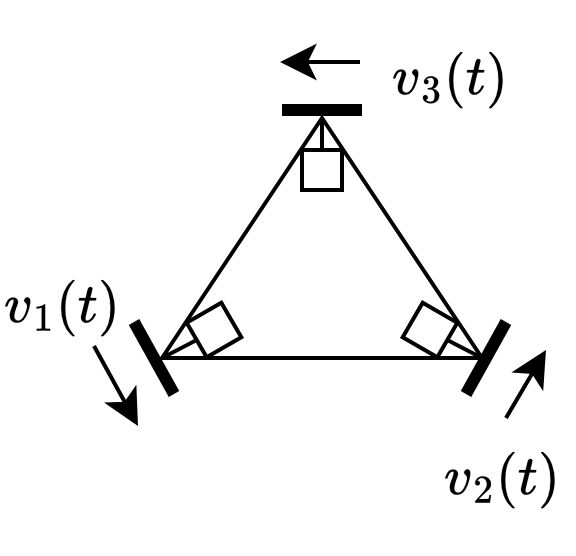
\includegraphics[width=0.25\linewidth]{images/omni.png} 
    \caption{Omnidirectional drive robot}
\end{figure}
To manipulate the robot's position, the following matrix governs its motion:
\[\begin{bmatrix}
    v_x \\ 
    v_y \\
    \dot{\theta} 
\end{bmatrix} = 
\begin{bmatrix}
    0 & -\frac{1}{\sqrt{3}}r & \frac{1}{\sqrt{3}}r \\
    -\frac{2}{3}r & \frac{1}{3}r & \frac{1}{3}r \\
    \frac{r}{3L} & \frac{r}{3L} & \frac{r}{3L}
\end{bmatrix}\begin{bmatrix}
    w_1 \\ 
    w_2 \\
    w_3 
\end{bmatrix}\]